\documentclass{beamer}
\usepackage{tikz}
\usepackage[all]{xy}
\usepackage{amsmath,amssymb}
\usepackage{hyperref}
\usepackage{graphicx}
\usepackage{algorithmic}
\usepackage{multirow}
 
\DeclareMathOperator*{\argmin}{arg\,min}
\DeclareMathOperator*{\Lik}{Lik}
\DeclareMathOperator*{\PoissonLoss}{PoissonLoss}
\DeclareMathOperator*{\Peaks}{Peaks}
\DeclareMathOperator*{\Segments}{Segments}
\DeclareMathOperator*{\argmax}{arg\,max}
\DeclareMathOperator*{\maximize}{maximize}
\DeclareMathOperator*{\minimize}{minimize}
\newcommand{\sign}{\operatorname{sign}}
\newcommand{\RR}{\mathbb R}
\newcommand{\ZZ}{\mathbb Z}
\newcommand{\NN}{\mathbb N}
\newcommand{\z}{$z = 2, 4, 3, 5, 1$} 

\newcommand{\algo}[1]{\textcolor{#1}{#1}}
\definecolor{PDPA}{HTML}{66C2A5}
\definecolor{CDPA}{HTML}{FC8D62}
\definecolor{GPDPA}{HTML}{4D4D4D}

% Set transparency of non-highlighted sections in the table of
% contents slide.
\setbeamertemplate{section in toc shaded}[default][100]
\AtBeginSection[]
{
  \setbeamercolor{section in toc}{fg=red} 
  \setbeamercolor{section in toc shaded}{fg=black} 
  \begin{frame}
    \tableofcontents[currentsection]
  \end{frame}
}

\begin{document}

\title{Validation croisée / cross-validation}

\author{
  Toby Dylan Hocking\\
  toby.dylan.hocking@usherbrooke.ca\\
}

\maketitle

\begin{frame}
  \frametitle{La validation croisée}
  Les données sont divisées en :
  \begin{itemize}
  \item train = entraînement, utilisé pour apprendre la fonction de prévision $f$.
  \item test, utilisé pour évaluer la qualité de la fonction de prévision $f$.
  \end{itemize}
\end{frame}

\section{Sur-apprentissage et Sous-apprentissage}

\begin{frame}
  \frametitle{Bon apprentissage}
  \begin{itemize}
  \item Fonction de bonne complexité (polynome degré 2)
  \item Bon régularité, bon variabilité.
  \item \tiny \url{https://tdhock.github.io/2020-02-03-capacity-polynomial-degree/}
  \end{itemize}
  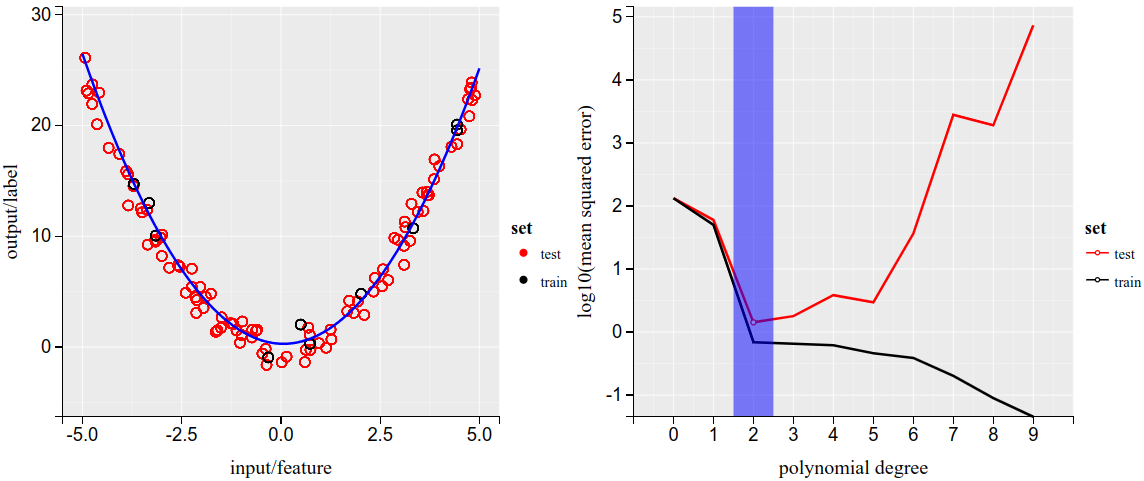
\includegraphics[width=\textwidth]{poly-good}
\end{frame}

\begin{frame}
  \frametitle{Sous-apprentissage}
  \begin{itemize}
  \item Fonction trop simple (polynome degré 1)
  \item Trop régulier, pas assez variable.
  \item \tiny \url{https://tdhock.github.io/2020-02-03-capacity-polynomial-degree/}
  \end{itemize}
  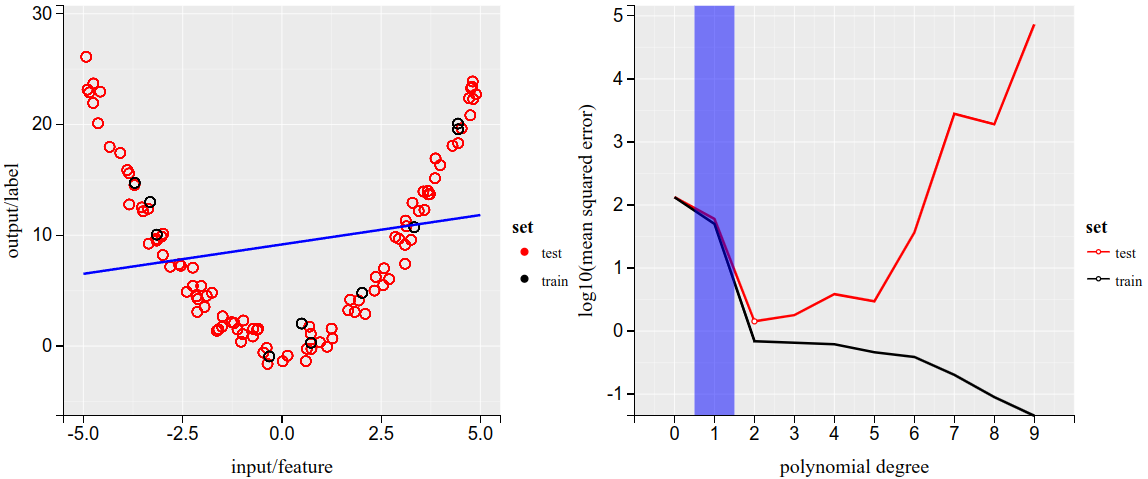
\includegraphics[width=\textwidth]{poly-under}
\end{frame}

\begin{frame}
  \frametitle{Sur-apprentissage}
  \begin{itemize}
  \item Fonction trop complexe (polynome degré 7)
  \item Pas assez régulier, trop variable.
  \item \tiny \url{https://tdhock.github.io/2020-02-03-capacity-polynomial-degree/}
  \end{itemize}
  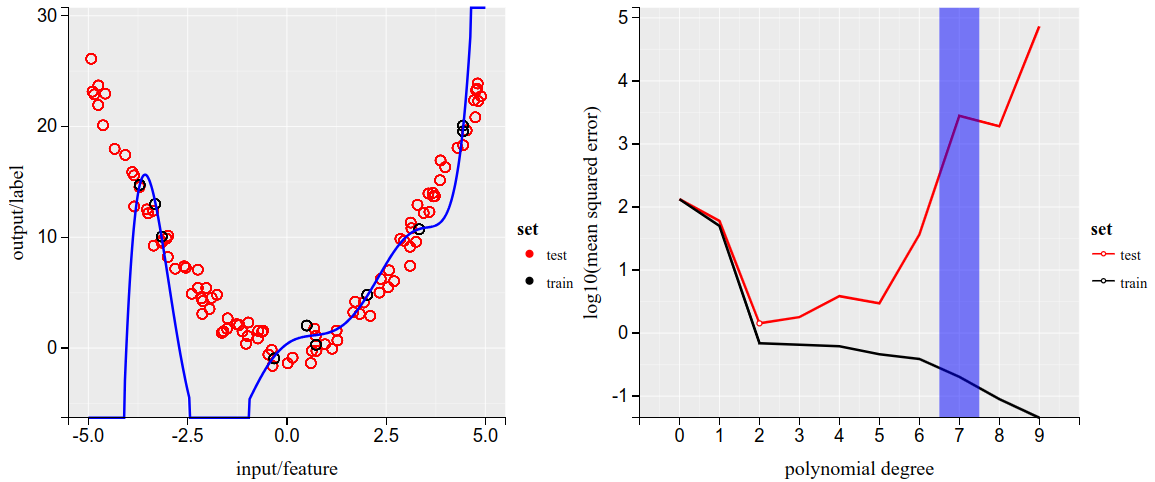
\includegraphics[width=\textwidth]{poly-overfit}
\end{frame}

\begin{frame}
  \frametitle{Sur- et Sous-apprentissage}
  \begin{itemize}
  \item \tiny \url{https://tdhock.github.io/2019-01-nearest-neighbor-regression-one-split/}
  \end{itemize}
  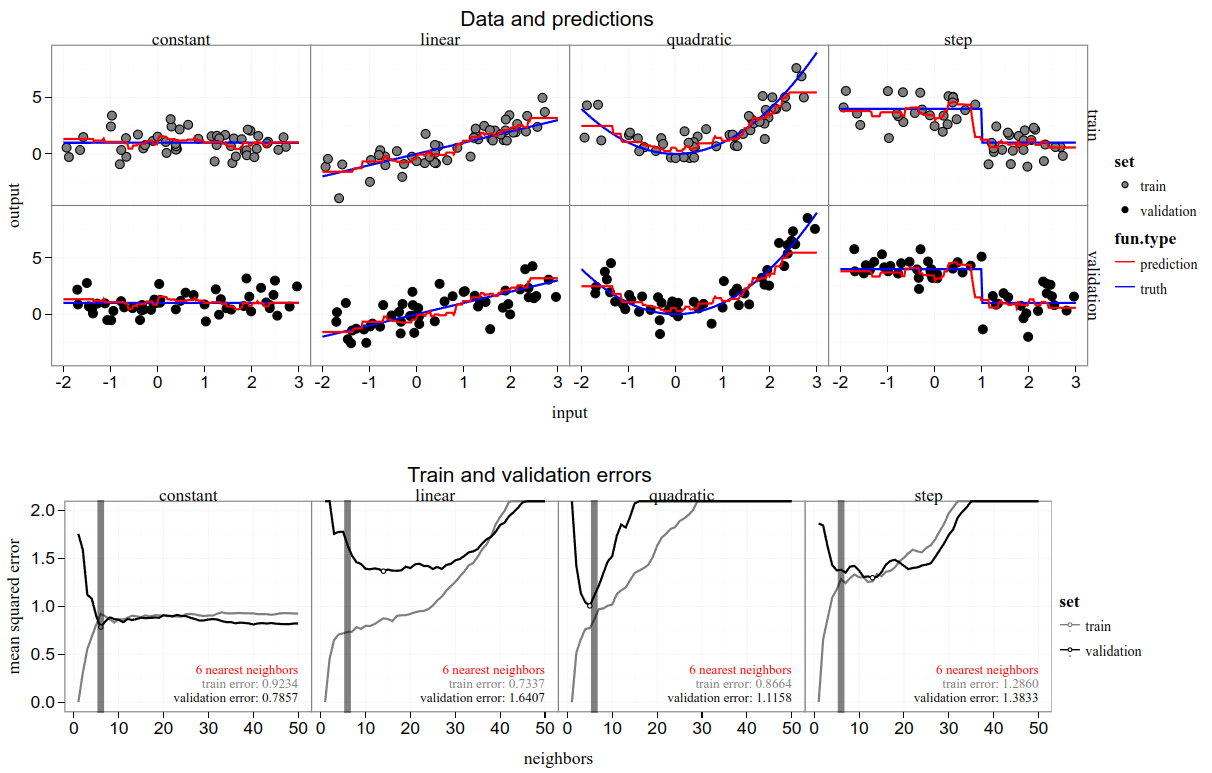
\includegraphics[width=\textwidth]{neighbors-4data}
\end{frame}

\section{Jeux de données standards}

\begin{frame}
  \frametitle{Classification d'images de chiffres (zipUSPS)}
  \begin{itemize}
  \item prop.correct = proportion correcte
  \item xgboost meilleur, mais voisins (nearest\_neighbors) est très
    proche... est-ce que la différence est significative ?
  \end{itemize}
  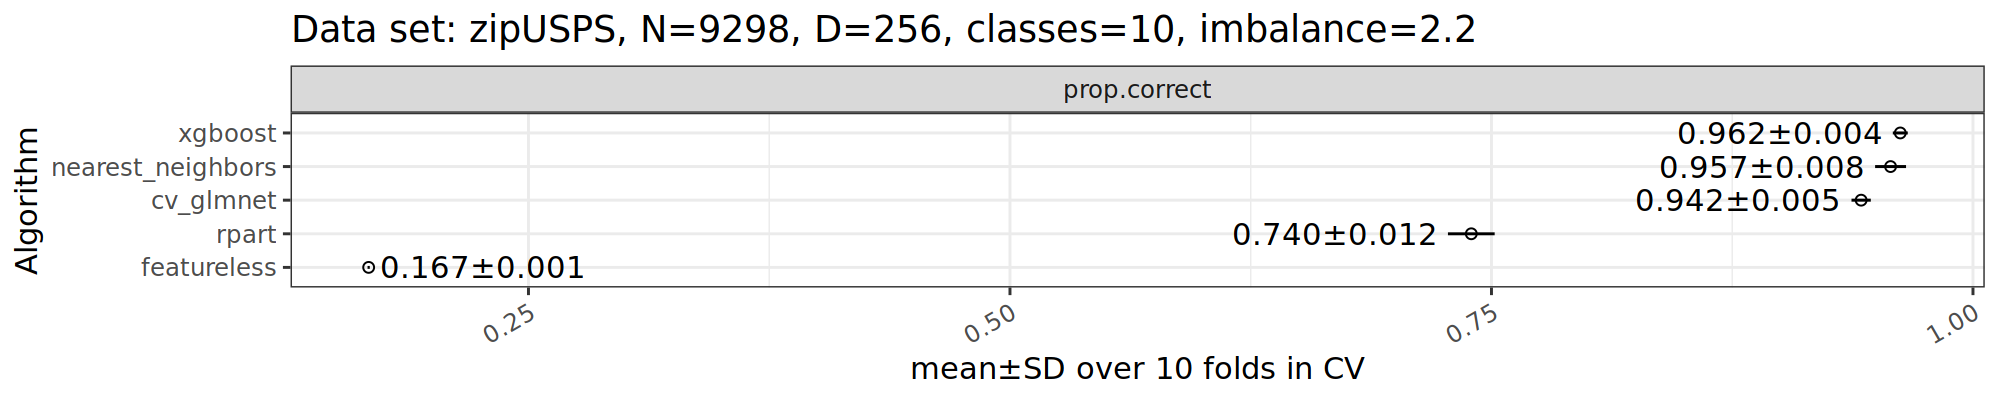
\includegraphics[width=\textwidth]{../cv-evaluation-examples/zipUSPS_error_algos_mean_SD.png}
\end{frame}

\begin{frame}
  \frametitle{Classification d'autisme}
  \begin{itemize}
  \item prop.correct = proportion correcte
  \item AUC = Area Under ROC Curve / Aire sous la courbe ROC (Taux de Vrai Positive vs. Taux de Faux Positive)
  \item xgboost meilleur, mais modèle linéaire (cv\_glmnet) est très
    proche... est-ce que la différence est significative ?
  \end{itemize}
  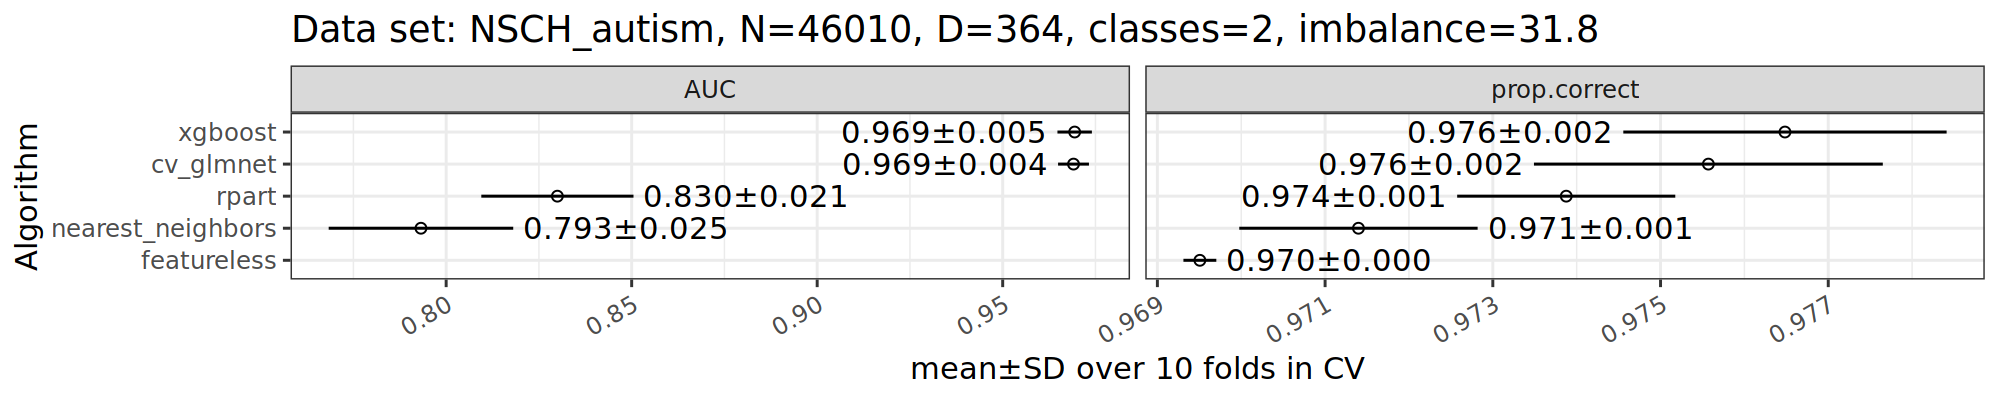
\includegraphics[width=\textwidth]{../cv-evaluation-examples/NSCH_autism_error_algos_mean_SD.png}
\end{frame}

\begin{frame}
  \frametitle{Visualisation du test de Student}
  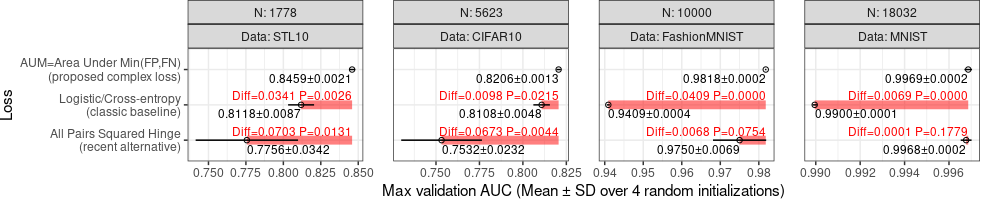
\includegraphics[width=2.9\textwidth]{p-others-1}
  \begin{itemize}
  \item X = Aire sous la courbe ROC.
  \item $p<0.05\Rightarrow$ différence significative.
  \item \tiny \url{https://tdhock.github.io/blog/2024/viz-pred-err/}
  \end{itemize}
\end{frame}

\begin{frame}
  \frametitle{Visualisation du test de Student}
  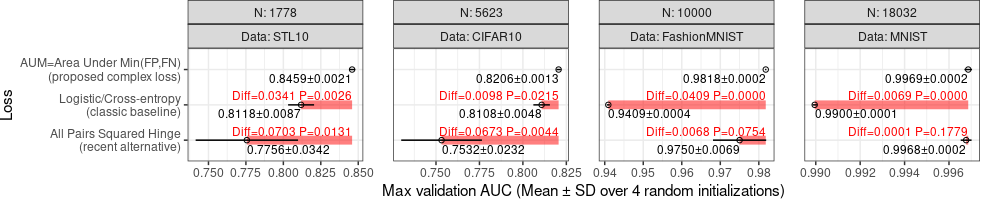
\includegraphics[width=\textwidth]{p-others-1}
  \begin{itemize}
  \item $p<0.05\Rightarrow$ différence significative.
  \item $p>0.05\Rightarrow$ différence non-significative.
  \item \tiny \url{https://tdhock.github.io/blog/2024/viz-pred-err/}
  \end{itemize}
\end{frame}

\begin{frame}
  \frametitle{Taux d'erreur et temps de calcul}
  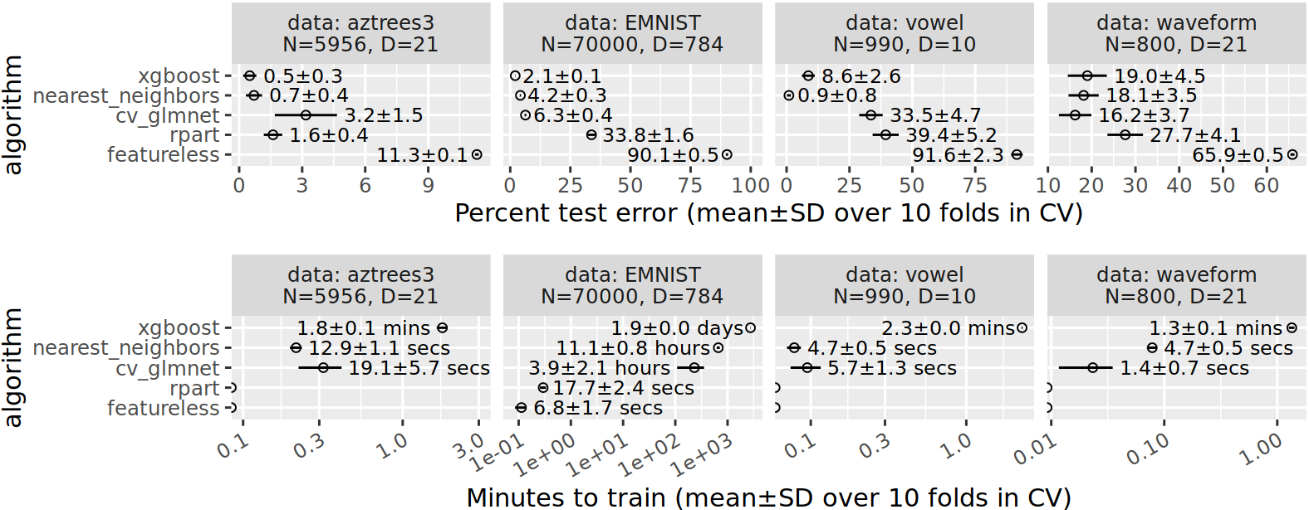
\includegraphics[width=\textwidth]{../cv-evaluation-examples/zz_error_minutes_4_data.png}
  \begin{itemize}
  \item featureless est le plus rapide, et toujours le plus erroné.  
  \item xgboost est le plus lent, le moins erroné dans aztrees3, EMNIST.
  \item Les plus proches voisins (nearest\_neighbors) est le meilleur dans vowel.
  \item Modèle linéaire (cv\_glmnet) est le meilleur dans waveform.
  \item Pour chaque jeu de données, on ne sait pas quel algo est
    préferable, jusqu'au moment de voir le résultat de la V-C.
  \end{itemize}
\end{frame}

\section{Simulations : quand est-ce que l'apprentissage est possible ? }

\begin{frame}
  \frametitle{Apprentissage facile / Easy learning}
  \begin{itemize}
  \item N=1000, bruit : facile, signal : sin.
  \item Erreur de rpart plus petit que featureless, $p<0.0001$
  \item \tiny \url{https://tdhock.github.io/2024-09-16-K-fold-CV-train-sizes-regression/}
  \end{itemize}
  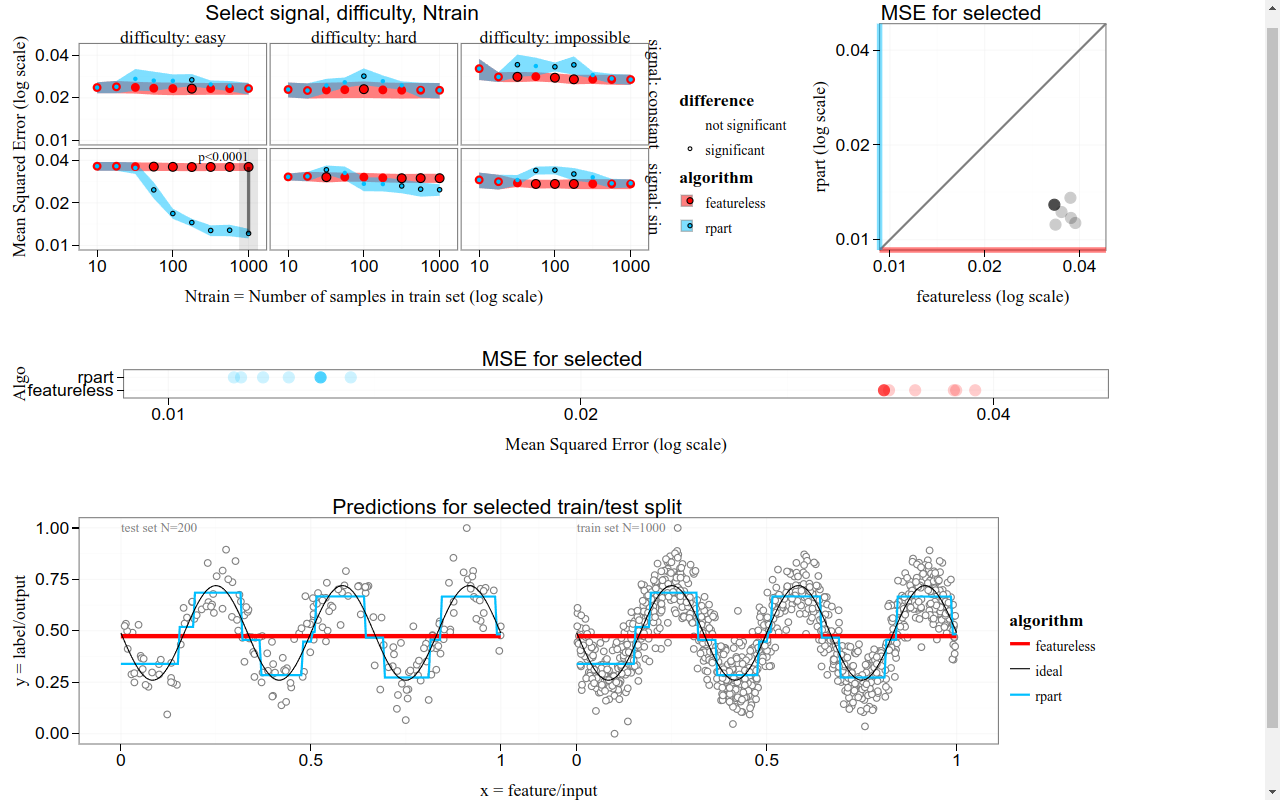
\includegraphics[width=\textwidth]{easy-1000}
\end{frame}

\begin{frame}
  \frametitle{Apprentissage possible / Possible learning}
  \begin{itemize}
  \item N=1000, bruit : dificile, signal : sin.
  \item Erreur de rpart plus petit que featureless, $p=0.0034$
  \item \tiny \url{https://tdhock.github.io/2024-09-16-K-fold-CV-train-sizes-regression/}
  \end{itemize}
  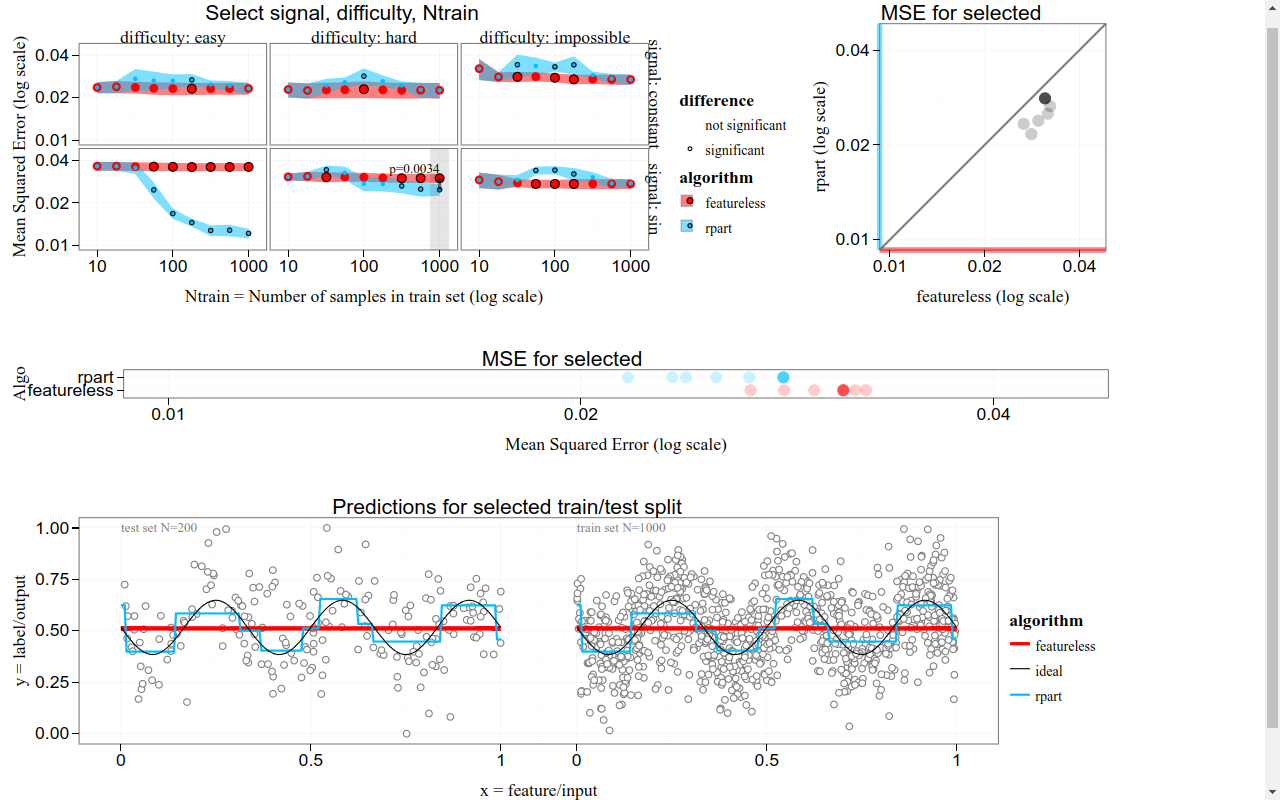
\includegraphics[width=\textwidth]{hard-1000}
\end{frame}

\begin{frame}
  \frametitle{Apprentissage impossible 1 / Impossible learning 1}
  \begin{itemize}
  \item N=1000, bruit : impossible, signal : sin.
  \item Erreur de rpart équivalent à featureless, $p=0.7620$.
  \item Mode d'échec 1 : trop de bruit / signal pas assez fort.
  \end{itemize}
  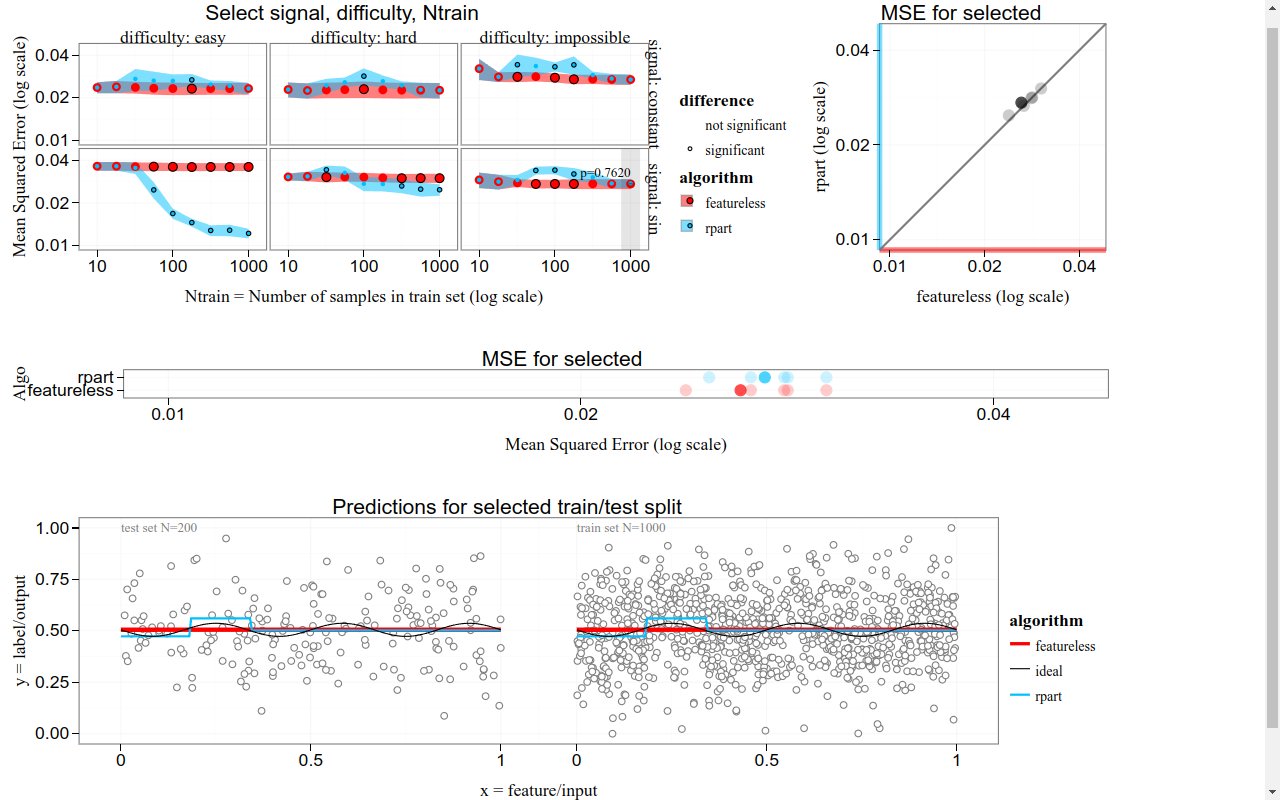
\includegraphics[width=\textwidth]{impossible-1000}
\end{frame}

\begin{frame}
  \frametitle{Apprentissage impossible 2 / Impossible learning 2}
  \begin{itemize}
  \item N=1000, bruit : facile, signal : constant.
  \item Erreur de rpart équivalent à featureless, $p=1$.
  \item Mode d'échec 2 : pas de rélation entre entrée $x$ et sortie $y$.
  \end{itemize}
  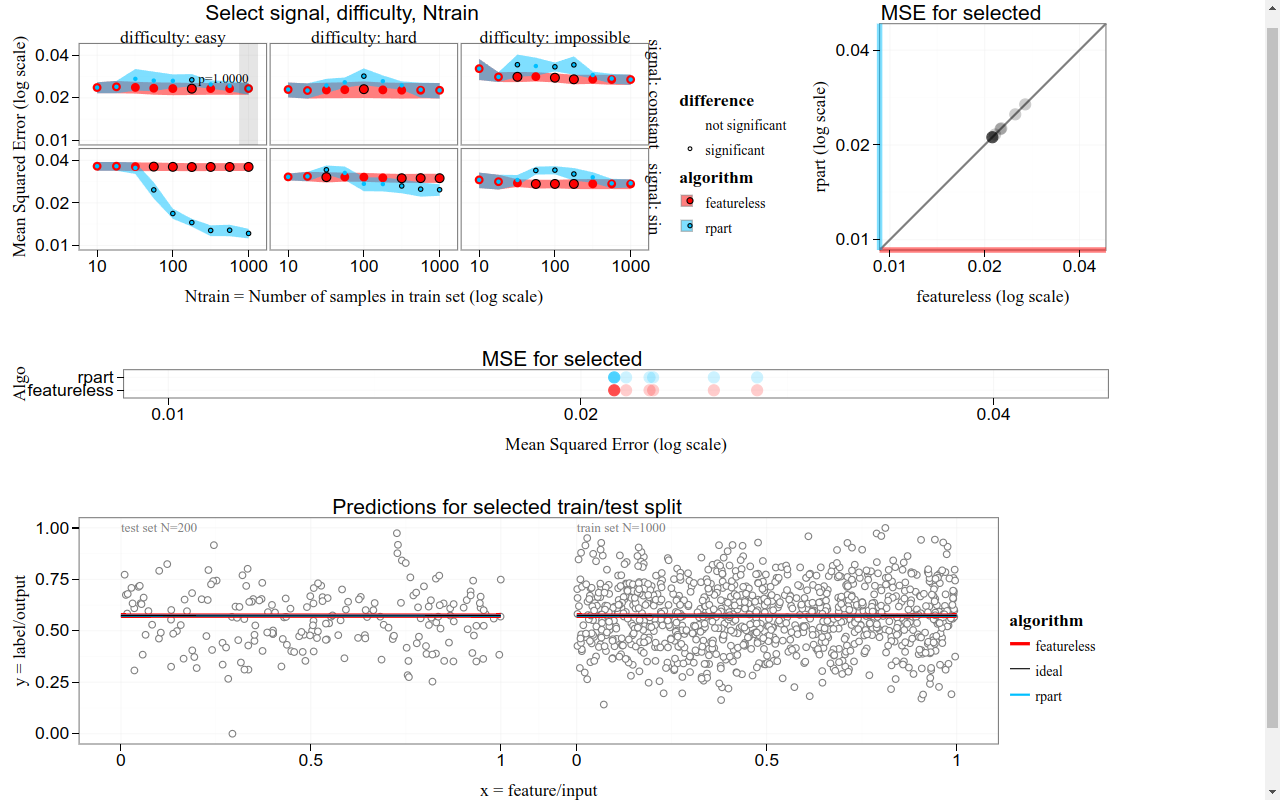
\includegraphics[width=\textwidth]{easy-1000-constant}
\end{frame}

\begin{frame}
  \frametitle{Apprentissage impossible 3 / Impossible learning 3}
  \begin{itemize}
  \item N=10, bruit : facile, signal : sin.
  \item Erreur de rpart équivalent à featureless, $p=1$.
  \item Mode d'échec 3 : pas assez de données.
  \end{itemize}
  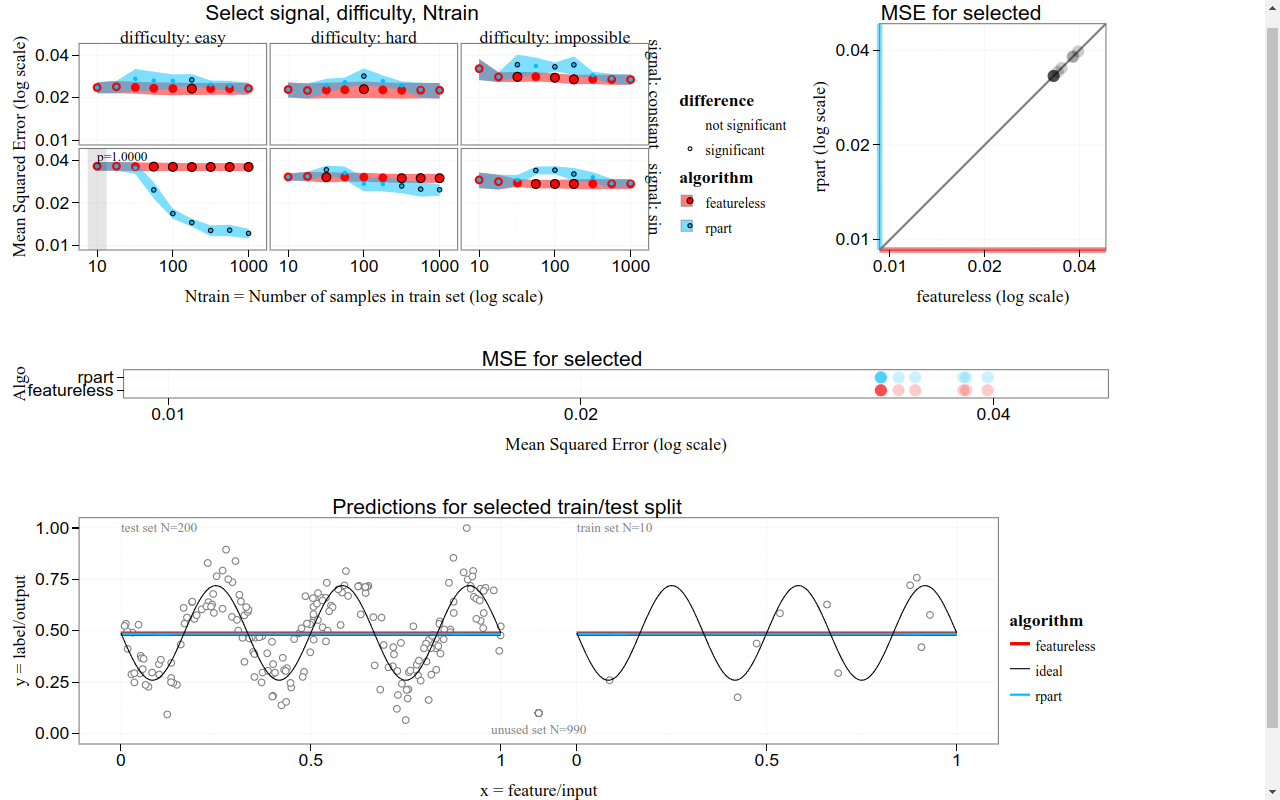
\includegraphics[width=\textwidth]{easy-10}
\end{frame}

\begin{frame}
  \frametitle{Sur-apprentissage / Overfitting}
  \begin{itemize}
  \item N=178, bruit : facile, signal : constant.
  \item Erreur de rpart plus grand featureless, $p=0.0325$.
  \item Mode d'échec 3 : pas assez de données.
  \end{itemize}
  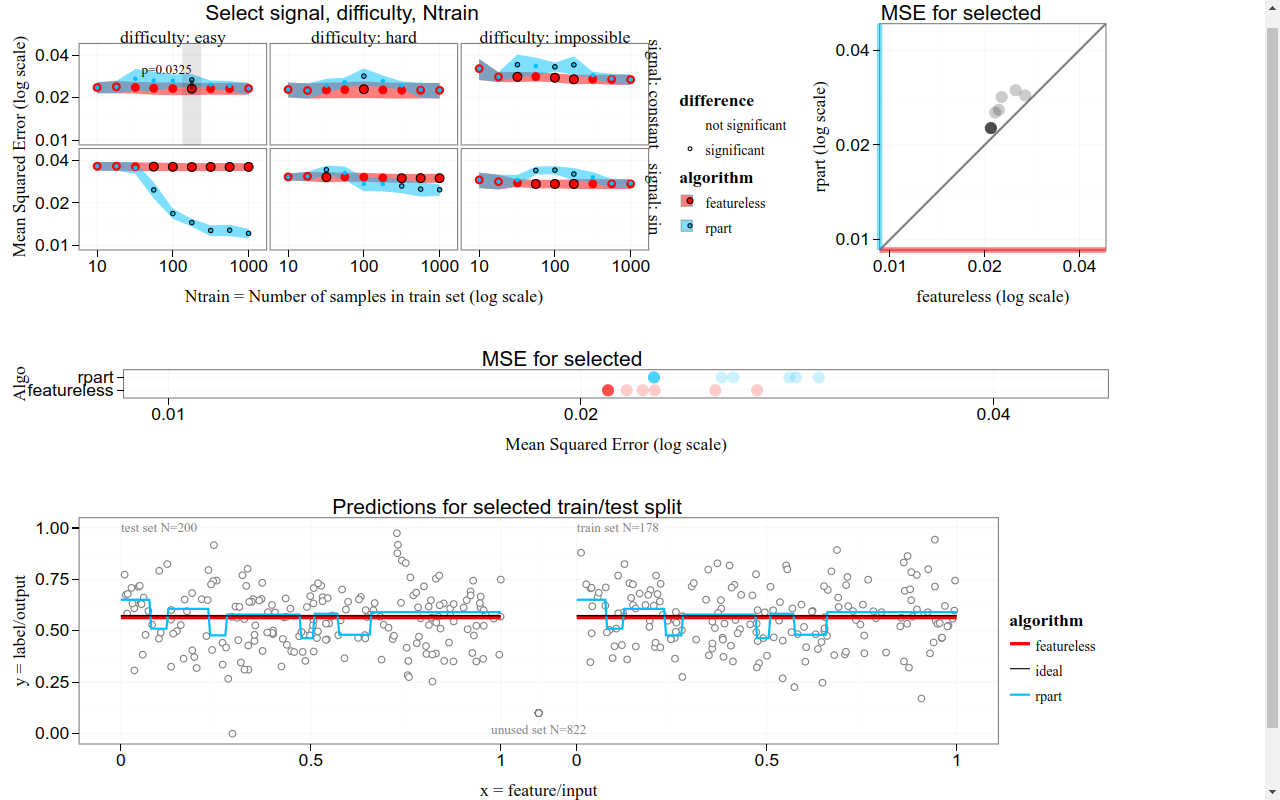
\includegraphics[width=\textwidth]{easy-overfit-constant}
\end{frame}



\end{document}
